%% Note that anything in a LaTeX file which is preceded (on the same line)
%% by a % is a comment, and is totally ignored by LaTeX.

%\documentclass[aps,prd,preprint]{revtex4}
\documentclass[aps,prd,final,twocolumn]{revtex4}

% Note:  comment out one of the two documentclass commands, depending
% on whether you need the final or preprint version. It is most convenient
% to work in preprint mode, and switch to final only at the end.

\usepackage{graphicx}                            % Graphics package
\usepackage{amsmath} 
\usepackage{tikz}
\usetikzlibrary{arrows,shapes}
\usetikzlibrary{trees}
\usepackage{lipsum} 
\usetikzlibrary{matrix,arrows} 	
\usepackage{mathtools}			
\usepackage{caption}
\usepackage{subcaption}
\captionsetup{compatibility=false} % for compatibility conflicts
%\captionsetup{justification=raggedright, singlelinecheck=false}
\captionsetup[figure]{justification=raggedright,singlelinecheck=false}
\captionsetup[subfigure]{justification=justified,singlelinecheck=false}
% For commutative diagram
											% http://www.felixl.de/commu.pdf
\usetikzlibrary{positioning}				% For "above of=" commands
\usetikzlibrary{calc,through}				% For coordinates
\usetikzlibrary{decorations.pathreplacing}  % For curly braces
% http://www.math.ucla.edu/~getreuer/tikz.html
\usepackage{pgffor}							% For repeating patterns

\usetikzlibrary{decorations.pathmorphing}	% For Feynman Diagrams
\usetikzlibrary{decorations.markings}
\tikzset{
	% >=stealth', %%  Uncomment for more conventional arrows
    vector/.style={decorate, decoration={snake}, draw},
	provector/.style={decorate, decoration={snake,amplitude=2.5pt}, draw},
	antivector/.style={decorate, decoration={snake,amplitude=-2.5pt}, draw},
    fermion/.style={draw=black, postaction={decorate},
        decoration={markings,mark=at position .55 with {\arrow[draw=black]{>}}}},
    fermionbar/.style={draw=black, postaction={decorate},
        decoration={markings,mark=at position .55 with {\arrow[draw=black]{<}}}},
    fermionnoarrow/.style={draw=black},
    gluon/.style={decorate, draw=black,
        decoration={coil,amplitude=4pt, segment length=5pt}},
    scalar/.style={dashed,draw=black},
    scalarbar/.style={dashed,draw=black, postaction={decorate},
        decoration={markings,mark=at position .55 with {\arrow[draw=black]{<}}}},
    scalarnoarrow/.style={dashed,draw=black},
    electron/.style={draw=black, postaction={decorate},
        decoration={markings,mark=at position .55 with {\arrow[draw=black]{>}}}},
	bigvector/.style={decorate, decoration={snake,amplitude=4pt}, draw},
}


%% The next few lines are definitions of commands used by Prof. Jaffe
%% when he wrote his paper.  The LaTeX-sophisticated among you
%% may have defined some labor-saving commands of your own.
%% If so, they go here.  The LaTeX-unsophisticated among you
%% may nevertheless want to use some of Prof. Jaffe's commands,
%% like \bra and \ket and \braket,  as done in the template below.
%% If you use these commands in your paper, keep their definitions
%% here.  If you do not use them, you can delete them.

\newcommand{\sech}{\mathop{\rm sech}\nolimits}
\newcommand{\bra}[1]{\left\langle #1 \right|}
\newcommand{\ket}[1]{\left|#1\right\rangle}
\newcommand{\braket}[2]{\left\langle#1 |  #2\right\rangle}
\newcommand{\rd}[1]{\mathop{\mathrm{d}#1}}
\newcommand{\refew}[1]{Eq.\eqref{eq:#1}}
\newcommand{\reffig}[1]{Fig. \ref{fig:#1}}
\newcommand{\refsec}[1]{Sec. \ref{sec:#1}}
\newcommand{\bsym}[1]{\boldsymbol{#1}}
\newcommand{\nn}[0]{\nonumber}
\newcommand{\note}[1]{\textcolor{orange}{#1}}
\newcommand{\notee}[1]{\textcolor{blue}{#1}}
\newcommand{\mm}[0]{\nonumber \\}
\newcommand{\ve}[0]{\varepsilon}
\newcommand{\nablav}[0]{\vec{\nabla}}

\allowdisplaybreaks

%%%%%%%%%%%%%%%


\begin{document}

\title{MCMC Solver on Planck 2015 High-$\ell$ $C_{\ell}^{TT}$}
\author{Alexander~Nie}
\affiliation{Harvard University,
28 Dewolfe St.,
Cambridge, MA 02138}
\date{December 7, 2016} 

\begin{abstract}
\noindent	
%\textbf{(Version 1: 12/8/2016)} 
In this project, an MCMC solver was implemented to estimate six cosmological parameters ($H_0$, $\Omega_b h^2$, $\Omega_{CDM} h^2$, $\tau$, $n_s$, and $A_s$) from the two-point angular power spectrum of temperature data from the Planck 2015 release. In contrast with standard MCMC solvers which use the Metropolis-Hastings algorithm, this project used an optimization known as \texttt{emcee} in order to optimize exploration of the possible values of the cosmological parameters. Using the high-$\ell$ data, the maximum likelihood estimates of the six-parameter set was $H_0 = 65.22\pm 11.08$, $\Omega_b^2 = .02193\pm .00437$, $\Omega_ch^2 = .1389\pm .1389$, $\tau = .08178\pm .03291$, $n_s = .9602\pm .0698$, $A_s = 2.212\times 10^9\pm .204\times 10^9$, in agreement with the existing literature.
 \end{abstract}

\maketitle

\pagestyle{myheadings}
\markboth{A. Nie}{Physics 212: Cosmology}
\thispagestyle{empty}


\section{Introduction}
\indent Modern cosmology faces a desirable, yet daunting problem: given the vast observational data made possible by increasingly large surveys, how can reliable statistical analyses be performed in a timely manner? One such solution to this problem are Markov-Chain Monte Carlo solvers, a class of algorithms which use random walks to sample the probability space of possible parameter values. In turn, this allows the solver to estimate aggregate properties of the sample without necessarily having to examine every single point in parameter space.

\indent For this project, six cosmological parameters, $H_0$, $\Omega_b h^2$, $\Omega_{CDM} h^2$, $\tau$, $n_s$, $A_s$, are varied near their fiducial values in the standard $\Lambda-$CDM cosmological model. Using a Boltzmann solver to predict the angular power spectrum $C_{\ell}$ of the Cosmic Microwave Background at each given value of the cosmological parameters, the likelihood of each cosmology can be computed by comparing against existing data from the Planck 2015 data release. Aggregate quantities such as the mean, variance, and covariance of the parameters are then estimated on the samples.

\section{Theoretical Foundations \label{sec:theory} }
\subsection{CMB Power Spectrum and Temperature}
To nearly $1$ in $10000$ parts, the Cosmic Microwave Background is a homogeneous and isotropic source of radiation[1]. However, small deviations from this isotropy in frequency, temperature, and polarization provide insight into the underlying cosmology. At early, radiation-dominant times in the universe, temperature deviations from isotropy largely originated from fluctuations in photon density $n_\gamma$. 

\begin{align}
\left(\frac{\delta\dot{n}_\gamma}{n\gamma}\right) &=-\nabla\cdot(\mathbf{v}\gamma)\label{lon1}\\
\nabla p_\gamma &= \frac{1}{3}\nabla \rho_\gamma\label{lon2}
\end{align}

Then from the continuity relation (\ref{lon1}), the equation of state on photons (\ref{lon2}), and the fact that $n_\gamma\propto T^3$, it can be shown that the angular power spectrum of temperature $\Theta$ in Fourier space obeys the harmonic oscillator equation [1]

\begin{align}
\ddot{\Theta}+\frac{1}{3}k^2\Theta = 0\label{lon3}
\end{align}

Assumining minimal initial velocities, the temperature power spectrum thus obeys

\begin{align}
\Theta(\eta_{recomb}) = \Theta(0)\cos(ks_{recomb})\label{lon4}
\end{align}

so peaks are expected to appear at $ks_{recomb}=1$ or characteristic scale $\lambda = \frac{2s}{n}$.

Decomposing $\Theta$ over the projected observational sphere into the spherical harmonics then yields coefficients of contribution whose two-point correlation functions are the power-spectrum $C_\ell$:

\begin{align}
\Theta(\hat{n}) &= \sum_{\ell=0}^\infty \sum_{m=-\ell}^{\ell} a_{\ell m}Y_{\ell m}(\hat{n}) \label{lon5}\\
\langle a_{\ell m} a_{\ell' m'}\rangle &= \delta_{\ell \ell'}\delta{m m'}C_{\ell}\\
C_{\ell} &= \frac{1}{2\ell+1}\sum_{m=-\ell}^\ell \langle |a_{\ell m}|^2\rangle \label{lon 7}
\end{align}

Thus, the $C_{\ell}$ encode the underlying dynamics of the cosmology expressed in temperature perturbations at a given scale in the CMB. For this project, $C_\ell^TT$ data was examined for $\ell>30$, as non-primordial perturbations, namely the Sachs-Wolfe effect, contribute to anisotropy at low $\ell$ [5]

\subsection{MCMC Solvers}
In a general Monte Carlo simulation, random samples are repeatedly taken in order to estimate some underlying distribution also known as the target distribution. In particular, the problem usually reduces to calculating some quantity
\begin{align}
\langle A\rangle = \frac{\sum_c A(c) e^{-\beta E(c)}}{Z}\label{lon8}
\end{align}

for a quantity $A$ dependent on the total configurations $c$ in the system, along with the weight of each configuration $0<e^{-\beta E(c)}<1$ and a normalization $Z=\sum_c e^{-\beta E(c)}$ [2]. In a uniform random sampling of all configurations, $\langle A\rangle$ can be estimated when $Z$ is known; however this simply creates a circular problem. 

In the Markov Chain solution to the problem, circularity is broken by sampling each configuration with dynamic probability $P(c,t)$ at time $g$ such that $P(c,t)\rightarrow \alpha e^{-\beta E(c)}$ for each configuration. In particular, at each time step, the probability distribution over the next configuration sampled depends only on the current configuration, endowing the solution with the Markov property. Then at equilibrium,
\begin{align}
P(c,\infty) &= \sum_{c'}T(c'\rightarrow c)P(c',\infty)\label{lon9}
\end{align}
where $T$ is the weight matrix. This condition imposes the detailed balance condition
\begin{align}
P(c',\infty) T(c'\rightarrow c) &= P(c,\infty)T(c\rightarrow c')\label{lon10}\\
\frac{T(c'\rightarrow c)}{T(c\rightarrow c')}&=e^{-\beta\Delta E}\label{lon11}
\end{align}
Thus, the probability of transition from a given configuration to the next is dependent only upon the ratio of the probabilities of transition. Equivalently, this means that at a given timestep, a new configuration should be automatically accepted when $\Delta E<0$ and accepted with a finite probability when $\Delta E>0$, giving rise to the Metropolis-Hastings algorithm for sampling (Sec. III). Assuming such an equilibrium state exists, then regardless of initial starting point in the parameter space, after a sufficiently long "burn-in" time, data aggregation should yield a reasonable estimate for the underlying parameter [2].

In a nutshell, $E$, the log probability is analogous to the "energy" of a probability landscape to be explored by the solver. Because all sampling occurs locally (only two configurations are calculated) rather than globally, this approach avoids the problem of enumerating all configurations in order to obtain a faithful estimate of the target distribution.

\subsection{Bayesian Methods}
Ultimately, the goal of the MCMC Solver in this project is to estimate the joint probability distributions of the six parameters given the observed data in $C_{\ell}$'s. This is equivalent to finding a posterior using Bayes' rule
\begin{align}
p(\mathbf{\theta}|\mathbf{x}) &= \frac{p(\mathbf{x}|\mathbf{\theta})p(\mathbf{\theta})}{p(\mathbf{x})}\label{lon12}
\end{align}

where $\theta$ is the parameters, $\mathbf{x}$ is the data, $p(\mathbf{x}|\theta)$ is the likelihood of seeing the data given a particular choice of parameters, and $p(\theta)$ is the prior: the probability of a particular choice of parameters based on some previous insight. As the data do not change and their underlying probabilities are unknown, the relation is often written $p(\theta|\mathbf{x})\propto p(\mathbf{x}|\theta)p(\theta)$ [3].

Assuming Gaussian error in the measurement, the likelihood for a given set of parameters is then calculated on the predicted $\hat{C}_{\ell}$'s against the measured $C_{\ell}$'s:
\begin{align}
p(\{C_{\ell}\}|\{\hat{C}_{\ell}\},\theta) &=\prod_{\ell} \frac{1}{\sigma_{C_{\ell}}\sqrt{2\pi}}\exp\left(-\frac{(\hat{C}_{\ell}-C_{\ell})^2}{2\sigma_{C_{\ell}}^2}\right)\label{lon13}
\end{align}

\section{Methods \label{sec:methods} }

\subsection{Metropolis-Hastings Algorithm}
As mentioned in \refsec{theory}, the asymptotic behavior of the Metropolis-Hastings algorithm depends on the random choice of configuration at timestep $t+1$ given only the current configuration $t$. In particular, if $E(C)$ is the log likelihood of a configuration $C$ (a particular set of values for the six cosmological parameters), then after samples $C$ at time $t$, the algorithm samples $C'$ with probability
\[min\left(e^{-E(C')-E(C)},1\right)\]

In the event $C'$ is not sampled, the algorithm then resamples $C$ at timestep $t+1$. The following describes the overall scheme of the algorithm[2,4]:

1. Pick some initial configuration (set of values) for the cosmological parameters $(H_0, \Omega_b h^2, \Omega_{CDM} h^2, \tau, n_s, A_s)$ in allowed parameter space.

2. Calculate the posterior of the configuration using the priors on the cosmological parameters and the likelihood on $C_{\ell}$.

3. Choose a configuration local to the current configuration with the probability scheme detailed above.

3. Cycle between 2 and 3 until the algorithm reaches equilibrium at which point the sampling should stop drifting.

4. Discard samples from earlier timesteps in which non-equilibrium occurs and calculate statistical quantities for the remaining data.

\subsection{Stretch-Move Optimization}
While the Metropolis-Hastings algorithm provides significant increases in computational efficiency over total enumeration of the parameter space, this project used a modification by Mackey et al. known as the "stretch-move" to further optimize the runtime efficiency [4]

To start, computation of the posterior at each configuration involves not only the likelihood, but also the prior. Although sufficiently long trials would asymptotically remove bias in the posterior from incorrect information in the prior, for $N$ parameters, even a simple multivariate Gaussian prior has $~N^2$ degrees of freedom in its covariance matrix. By using an affine invariant algorithm, an algorithm that is invariant under linear transformation of the data, the MCMC solver becomes sensitive only to the $N$ diagonal terms of the covariance matrix as the system can be rotated into one for which variation occurs only along principal axes. This then reduces the degrees of freedom (and thus guesswork) needed for initializing a prior.[4]

Second, the Metropolis-Hastings algorithm examines a single configuration at a time. Imagining the algorithm as  "walker" between points of parameter space, the locality of MCMC methods means that a single "walker" will need quite a bit of time to sufficiently explore parameter space while multiple walkers under the Metropolis-Hastings algorithm are independent, so their data cannot be aggregated. Under the stretch-move algorithm proposed by Mackey et al., this idea is better optimized by having an ensemble of walkers, leading to parallelizability. Therefore, although the number of samples and computations remains approximately the same, this algorithm allows shorter wait-times when parallelized.

 The algorithm is as follows[4]:

1. Pick several initial configurations to serve as starting points for different walkers in two ensembles of $K$ walkers, $S_K$ and $S'_K$.

2. At time $t$, randomly pick a walkers $X_k$,$X'_k$ from the ensembles $S_K,S'_K$, a random number $z$ from the unit interval.

3. Move $X_k$ $z(X_k-X_k')$ along the line segment between $X_k$ and $X_k'$  in parameter space to a new configuration $Y$

4. Accept and sample the new configuration with the probability scheme $P(accept) = z^{N-1}\frac{p(Y)}{p(X_k)}$ where $p(X)$ is the prior on that configuration. In the event of rejection, return $X_k$ to its original configuration at time $t$ and sample that configuration.

5. Repeat steps 2-4 to move walker in $X'_k$.

6. Repeat steps 2-5 until the position of the walkers stops drifting.

\subsection{Other Implementation Specifics}
The Boltzmann solver CAMB (Code for Anisotropies in the Microwave Background) was used to calculate predicted $\hat{C}_\ell$'s for each configuration of $(H_0, \Omega_b h^2, \Omega_{CDM}h^2, \tau, n_s, A_s)$, with all other values fixed to their best-fit values in the Planck collaboration (\ref{tab:table1}) and assuming an infinitesimal reionization depth. For the measured $C_{\ell}$'s, high-$\ell$ data and uncertainties were taken from the Planck Legacy Archive[5,6]. Following the Planck collaboration, a Gaussian prior was used for $\tau$ while the tophat prior was used for the other five cosmological parameters studied[5]. Finally, the project implemented a multi-threaded version with a small number of walkers intended for a quad-core laptop and an MPI-based version with a large number of walkers intended for the Harvard ODYSSEY cluster.

\begin{table}
\caption{\label{tab:table1} Priors and fixed values for various cosmological parameters used by CAMB}
\begin{tabular}{cc}
Parameter & Prior\\ 
\hline
 $H_0$ & $[40,100]$\\
 $\Omega_b h^2$ & $[0.005,0.1]$ \\
 $\Omega_{CDM} h^2$ &[.001,.99]\\
 $\tau$ & $\mathcal{N}(.07,.02)$\\
 $n_s$ & $[0.9,1.1]$\\
 $\ln(10^{10}A_s)$ & $[2.7,4.0]$\\
 \hline
   \label{tab:priors}
\end{tabular}
\end{table}

\section{Results and Discussion \label{sec:expanls} }

\subsection{High-$\ell$ $C_\ell$ Spectrum}

Two extended trials were run, one with 12 walkers over 700 steps (single node) and one with 16 walkers over 1600 steps (cluster). Results can be found in the Appendix.

Overall, both runs had significant overlap on values for the cosmological parameters. Examining the run data (FIG. 1, FIG. 2), however, showed that fewer walkers generally converged faster than more walkers. In particular, burn-in seems to occur at around 200 steps for the 12-walker trial and 600-steps for the 16-walker trial. This is most likely due to  overexploration of the parameter space by the trial with more walkers. In particular, a higher density of walkers implies a smaller distance between them. As the stretch-move causes walkers to jump configurations proportional to the distance between walkers, this causes the low-walker trial to have more jumps, thereby smoothing local behavior in the parameter space. As the acceptance fraction, the fraction of times a new configuration is sampled over the current one, was $.767$ for the 16-walker trial and $.344$ for the 12-walker trial, this supports the idea that a 16-walker trial might be too large a number of walkers for a six-parameter model.

Examining the corner plots (FIG. 3, FIG. 4), the 16-walker model showed much more ovoid features around the data peaks while the 12-walker model not only had greater spreads, but also managed to capture very elongated relationships. This again supports the idea that the 16-walker model might not be appropriate, as a high acceptance fraction generally means walkers are already concentrated near the maximum likelihood estimate, whereas the goal of the algorithm is to discover the distribution as well. 

\section{Conclusion}
MCMC Solvers offer a way to faithfully estimate an underlying target distribution. From the Monte Carlo property, the solvers avoid the problem of having to enumerate every possible point in the target distribution. From the Markov property, the solvers further reduce computation demand by strategically sampling local configurations, allowing for relatively small calculations. Combined with a Boltzmann solver, MCMC solvers are useful in cosmology as a way to explore the target distribution over various cosmological parameters without having to directly and simultaneously optimize the many parameters and equations governing cosmological evolution. Future steps for this project might involve implementing a Hamiltonian MC solver. Such a solver uses Hamiltonian equations with occasional kicks (ergodic evolution), rather than a Markov process (stochastic evolution) to decide amongst local configurations.

\section{Appendix}
\begin{figure*}
\begin{center}
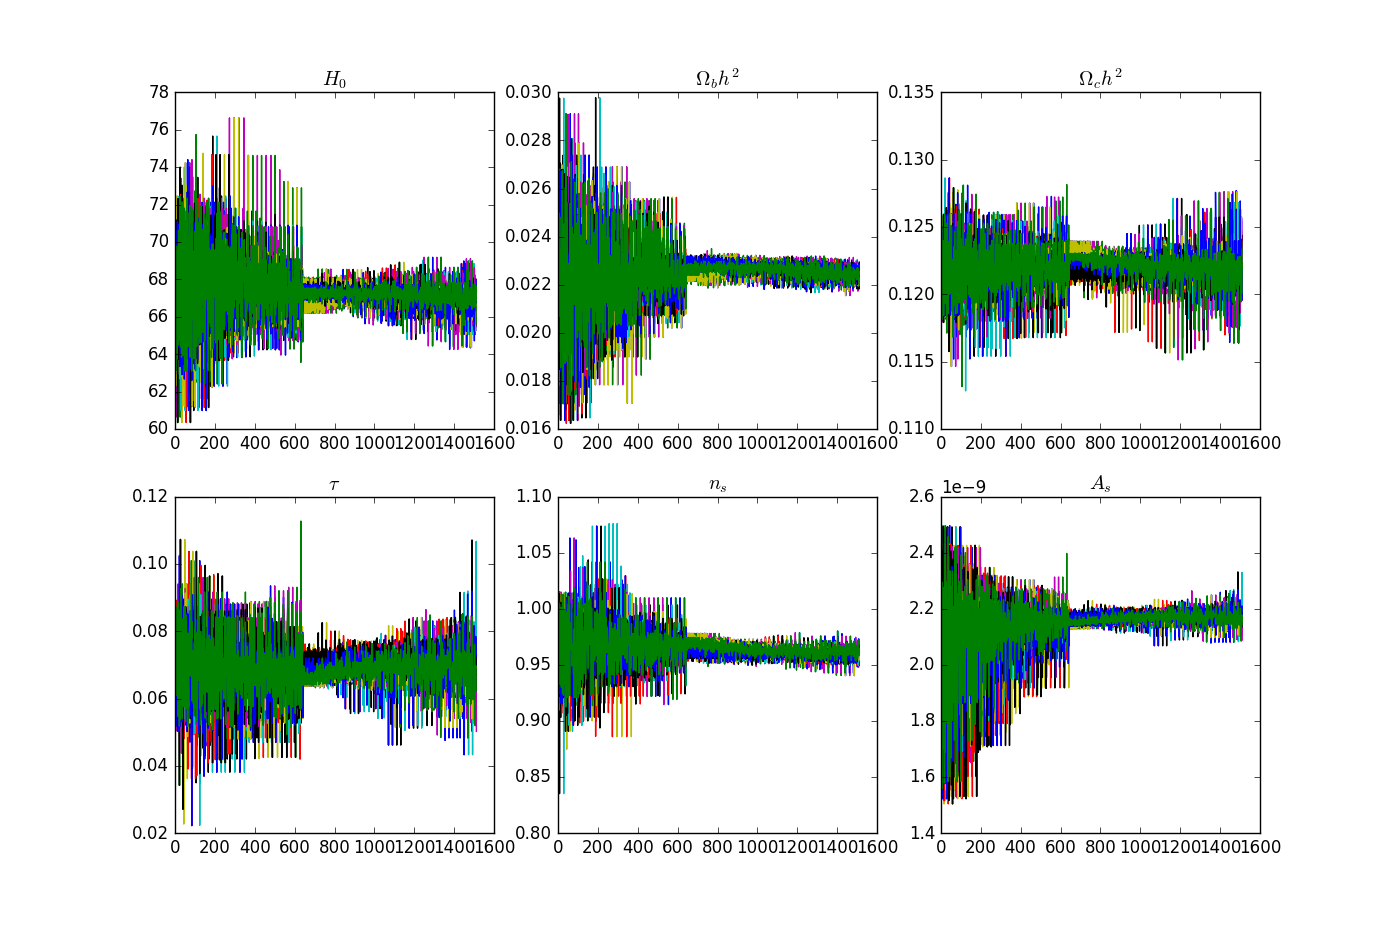
\includegraphics[scale=.4]{runs_16_800.png}
\label{fig:f1}
\caption{Walker Plot for the 16-walker, 1600-step trial}
\end{center}
\end{figure*}

\begin{figure*}
\begin{center}
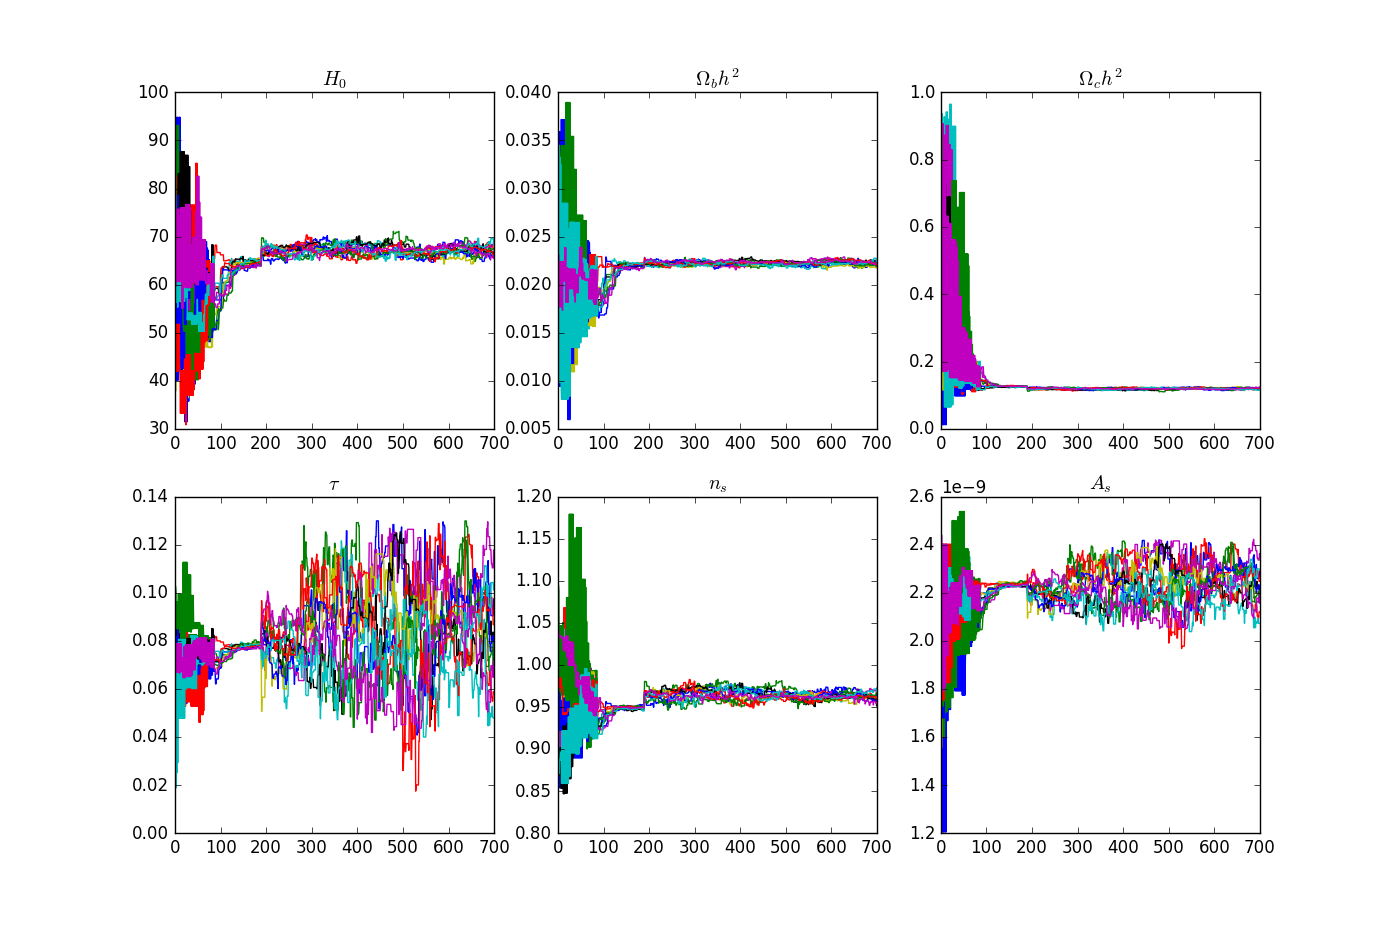
\includegraphics[scale=.4]{runs_12_700.png}
\label{fig:f2}
\caption{Walker Plot for the 12-walker, 700-step trial}
\end{center}
\end{figure*}

\begin{figure*}
\begin{center}
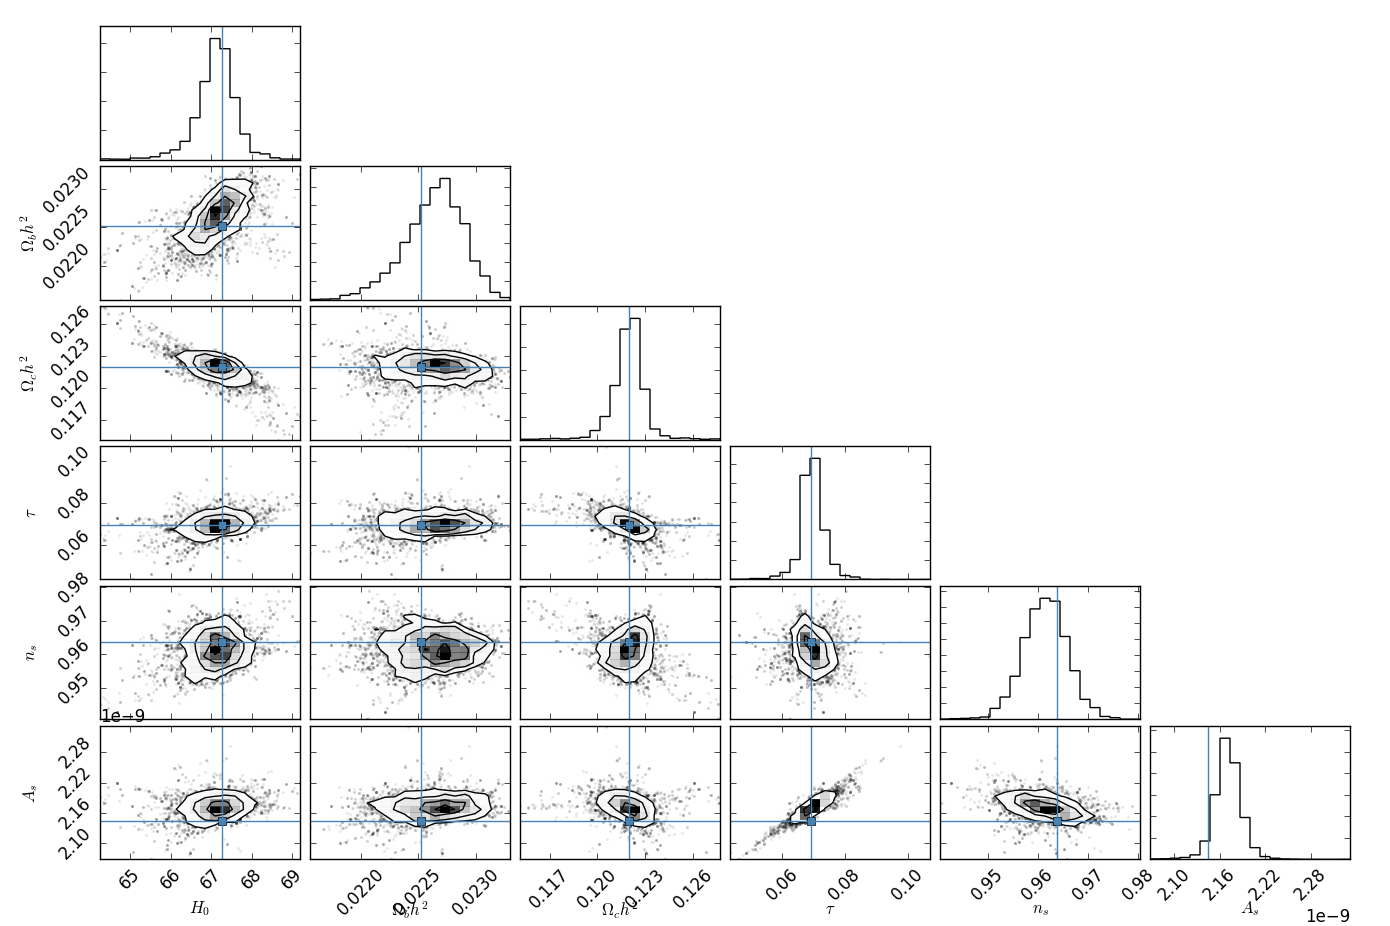
\includegraphics[scale=.4]{data_16_800.png}
\label{fig:f3}
\caption{Corner Plot for the 16-walker, 1600-step trial}
\end{center}
\end{figure*}

\begin{figure*}
\begin{center}
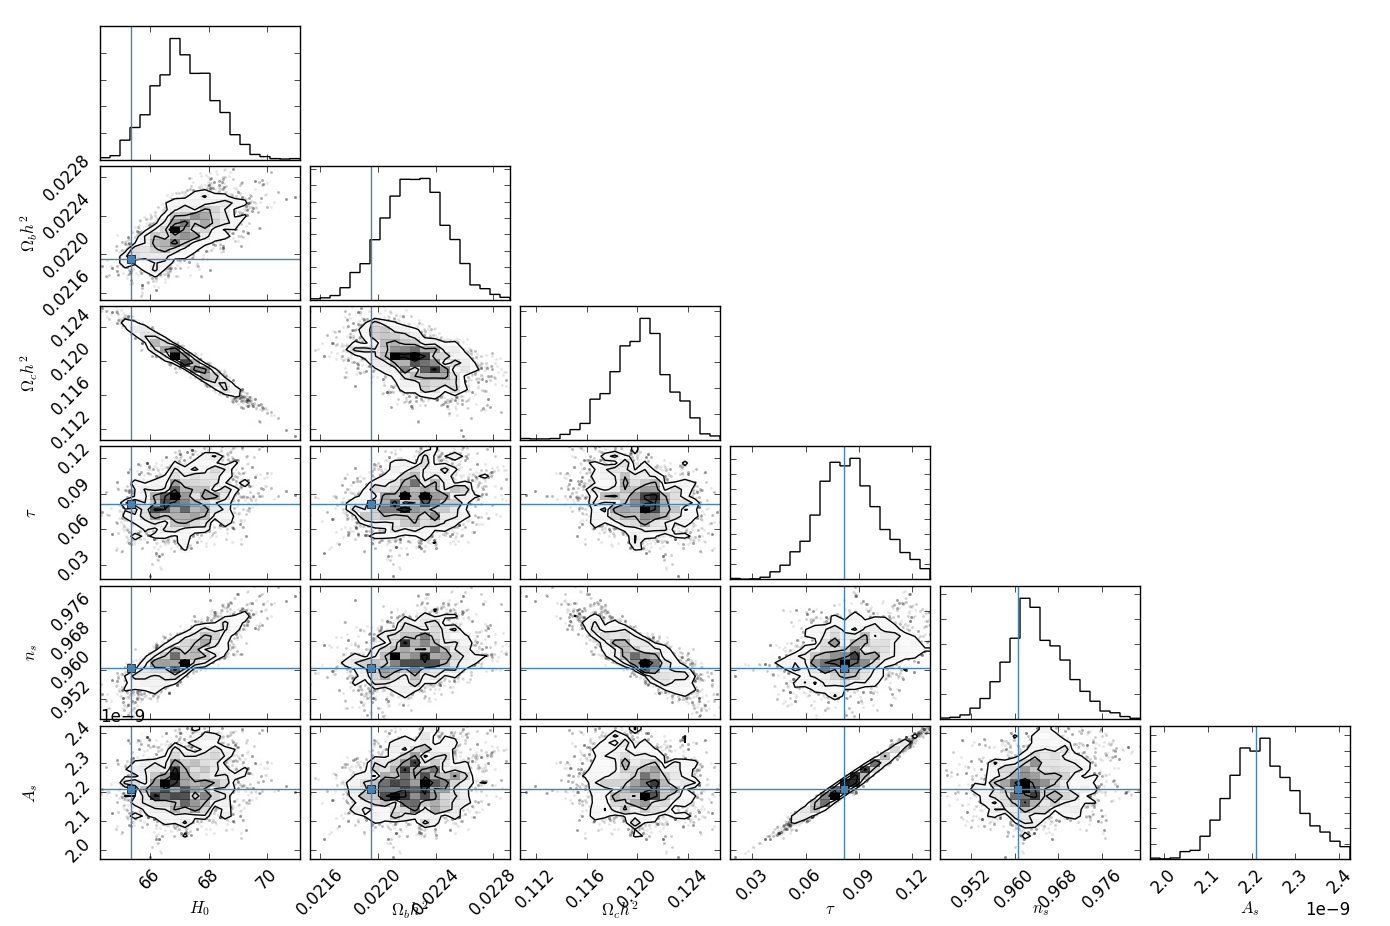
\includegraphics[scale=.4]{data_12_700.png}
\label{fig:f4}
\caption{Corner Plot for the 12-walker, 700-step trial}
\end{center}
\end{figure*}

\begin{figure*}
\begin{center}
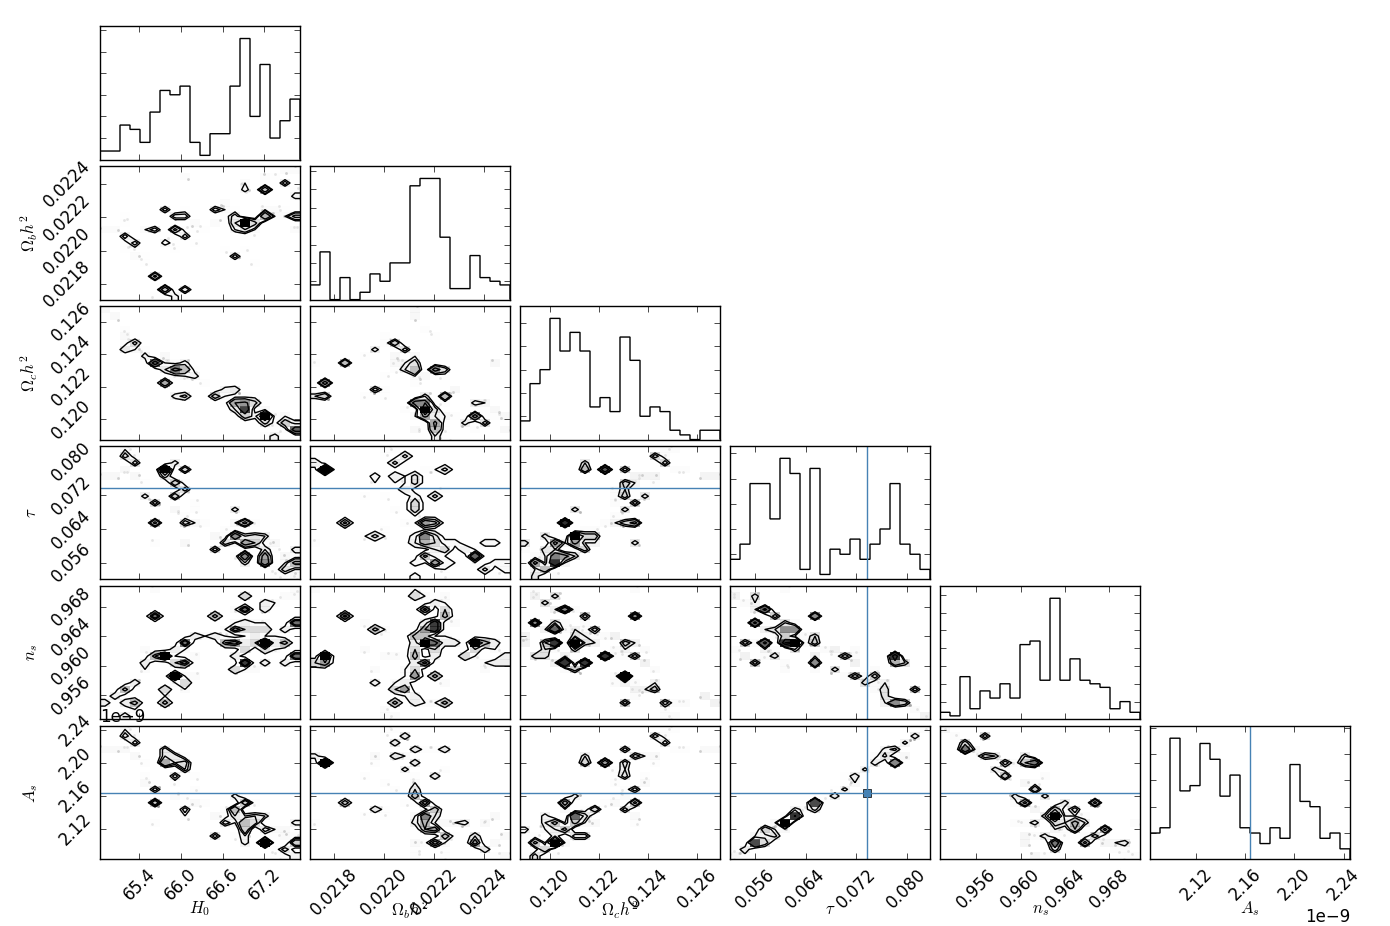
\includegraphics[scale=.4]{data_12_200.png}
\label{fig:f4}
\caption{A Bad Run: Corner Plot for the 12-walker, 200-step trial. Note the disjoint regions, which indicate the walkers have not had sufficient time to explore parameter space and settle near an optima.}
\end{center}
\end{figure*}
\begin{table*}
\caption{\label{tab:table3} Estimates of Cosmological Parameters from a 12-walker, 700-step and 16-walker, 1600-step MCMC trial. Uncertainties are given at the 68\% level.}
\begin{ruledtabular}
\begin{tabular}{ccccc}
 &\multicolumn{1}{c}{12-walker run}&\multicolumn{3}{c}{16-walker run }\\
Parameter & Max Likelihood Estimate  & $68\% bounds$ & Max Likelihood Estimate & $68\% bounds$
\\ \hline
 $H_0$&$65.22$ &$54.14-76.30$ &$67.27$ & $64.67-69.86$ \\
 $\Omega_b^2$& $.02193$  & $.01782-.02604$  & $.02252$ &  $.02033- .02471 $ \\
 $\Omega_c h^2$ &$.1389$ &$0-.3053$&$.1220$ & $.1193-.1247$ \\
 $\tau$ & $.08178 $&$04887-.14469$  &$ .06919$ & $.05557-.08281$ \\
 $n_s$&$.9602 $ &$ .9210-.9995$&$ .9637$ & $.9382-.9894$  \\
 $A_s$ & $2.212\times 10^{-9} $ & $2.008\times 10^{-9}-2.415\times 10^{-9}$ &$ 2.144\times 10^{-9}$ & $1.954\times 10^{-9}-2.334\times 10^{-9}$ \\
   \label{tab:main_data}
\end{tabular}
\end{ruledtabular}
\end{table*}

\subsection*{Acknowledgments}
 
The authors are grateful Prof. Cora Dvorkin and Tansu Daylan for both their assistance on the project and their wonderful teaching.

\bibliographystyle{ieeetr} 
\bibliography{phys212_2016}

\begin{thebibliography}{9}
\bibitem{ref:1.1} Tojeiro, R. 2006. \textit{Understanding the Cosmic Microwave Background Temperature Spectrum}
\bibitem{ref:1.2} Levine, E. 2015. \textit{Numerical Simulations}
\bibitem{ref:1.3} Mackey et al., 2013. \textit{emcee: The MCMC Hammer}
\bibitem{ref:1.4} Heavens, A. 2001. \textit{Statistics in Cosmology}
\bibitem{ref:1.5} Planck Collaboration: \textit{Planck} 2015 results. XIII
\bibitem{ref:1.6} www.pla.esac.esa.int
\end{thebibliography}

\end{document}
